\hypertarget{_mag_step_8c}{
\section{/home/mgh/LanlGeoMag/libLanlGeoMag/MagStep.c File Reference}
\label{_mag_step_8c}\index{/home/mgh/LanlGeoMag/libLanlGeoMag/MagStep.c@{/home/mgh/LanlGeoMag/libLanlGeoMag/MagStep.c}}
}
{\tt \#include \char`\"{}Lgm/Lgm\_\-MagModelInfo.h\char`\"{}}\par


Include dependency graph for MagStep.c:\nopagebreak
\begin{figure}[H]
\begin{center}
\leavevmode
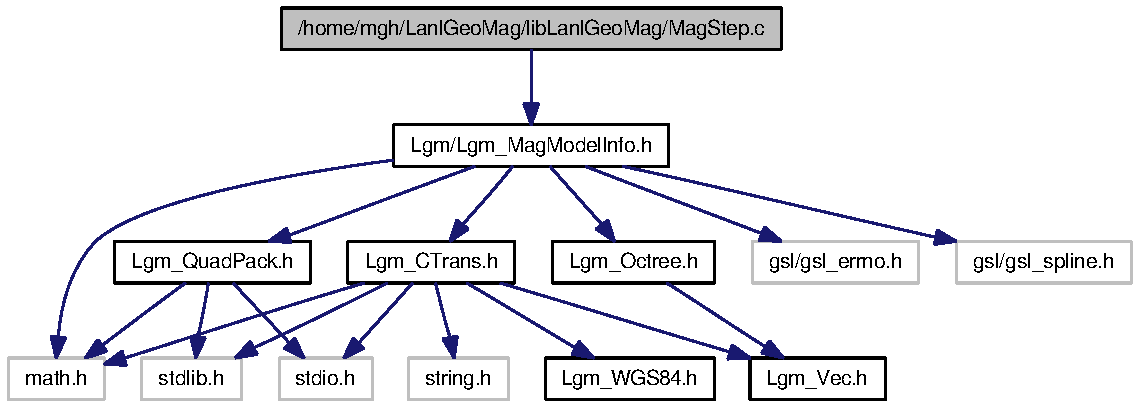
\includegraphics[width=291pt]{_mag_step_8c__incl}
\end{center}
\end{figure}
\subsection*{Functions}
\begin{CompactItemize}
\item 
void \hyperlink{_mag_step_8c_25b0aafbfa7b08a20caa7103067395eb}{Lgm\_\-ModMid} (\hyperlink{struct_lgm___vector}{Lgm\_\-Vector} $\ast$u, \hyperlink{struct_lgm___vector}{Lgm\_\-Vector} $\ast$v, double H, int n, double sgn, int($\ast$Mag)(\hyperlink{struct_lgm___vector}{Lgm\_\-Vector} $\ast$, \hyperlink{struct_lgm___vector}{Lgm\_\-Vector} $\ast$, \hyperlink{struct_lgm___mag_model_info}{Lgm\_\-MagModelInfo} $\ast$), \hyperlink{struct_lgm___mag_model_info}{Lgm\_\-MagModelInfo} $\ast$Info)
\item 
void \hyperlink{_mag_step_8c_e3bb72fc4563ef180d82d4cc003bcf0e}{Lgm\_\-RatFunExt} (int k, double x\_\-k, \hyperlink{struct_lgm___vector}{Lgm\_\-Vector} $\ast$u\_\-k, \hyperlink{struct_lgm___vector}{Lgm\_\-Vector} $\ast$w, \hyperlink{struct_lgm___vector}{Lgm\_\-Vector} $\ast$dw, \hyperlink{struct_lgm___mag_model_info}{Lgm\_\-MagModelInfo} $\ast$Info)
\item 
int \hyperlink{_mag_step_8c_3b19333caf8b3d06e1b4c54e4473096b}{Lgm\_\-MagStep} (\hyperlink{struct_lgm___vector}{Lgm\_\-Vector} $\ast$u, \hyperlink{struct_lgm___vector}{Lgm\_\-Vector} $\ast$u\_\-scale, double Htry, double $\ast$Hdid, double $\ast$Hnext, double eps, double sgn, double $\ast$s, int $\ast$reset, int($\ast$Mag)(\hyperlink{struct_lgm___vector}{Lgm\_\-Vector} $\ast$, \hyperlink{struct_lgm___vector}{Lgm\_\-Vector} $\ast$, \hyperlink{struct_lgm___mag_model_info}{Lgm\_\-MagModelInfo} $\ast$), \hyperlink{struct_lgm___mag_model_info}{Lgm\_\-MagModelInfo} $\ast$Info)
\end{CompactItemize}


\subsection{Function Documentation}
\hypertarget{_mag_step_8c_25b0aafbfa7b08a20caa7103067395eb}{
\index{MagStep.c@{MagStep.c}!Lgm\_\-ModMid@{Lgm\_\-ModMid}}
\index{Lgm\_\-ModMid@{Lgm\_\-ModMid}!MagStep.c@{MagStep.c}}
\subsubsection[{Lgm\_\-ModMid}]{\setlength{\rightskip}{0pt plus 5cm}void Lgm\_\-ModMid ({\bf Lgm\_\-Vector} $\ast$ {\em u}, \/  {\bf Lgm\_\-Vector} $\ast$ {\em v}, \/  double {\em H}, \/  int {\em n}, \/  double {\em sgn}, \/  int($\ast$)({\bf Lgm\_\-Vector} $\ast$, {\bf Lgm\_\-Vector} $\ast$, {\bf Lgm\_\-MagModelInfo} $\ast$) {\em Mag}, \/  {\bf Lgm\_\-MagModelInfo} $\ast$ {\em Info})}}
\label{_mag_step_8c_25b0aafbfa7b08a20caa7103067395eb}




Definition at line 17 of file MagStep.c.

Here is the call graph for this function:\nopagebreak
\begin{figure}[H]
\begin{center}
\leavevmode
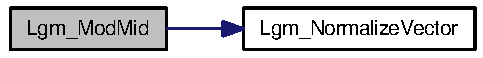
\includegraphics[width=134pt]{_mag_step_8c_25b0aafbfa7b08a20caa7103067395eb_cgraph}
\end{center}
\end{figure}


Here is the caller graph for this function:\nopagebreak
\begin{figure}[H]
\begin{center}
\leavevmode
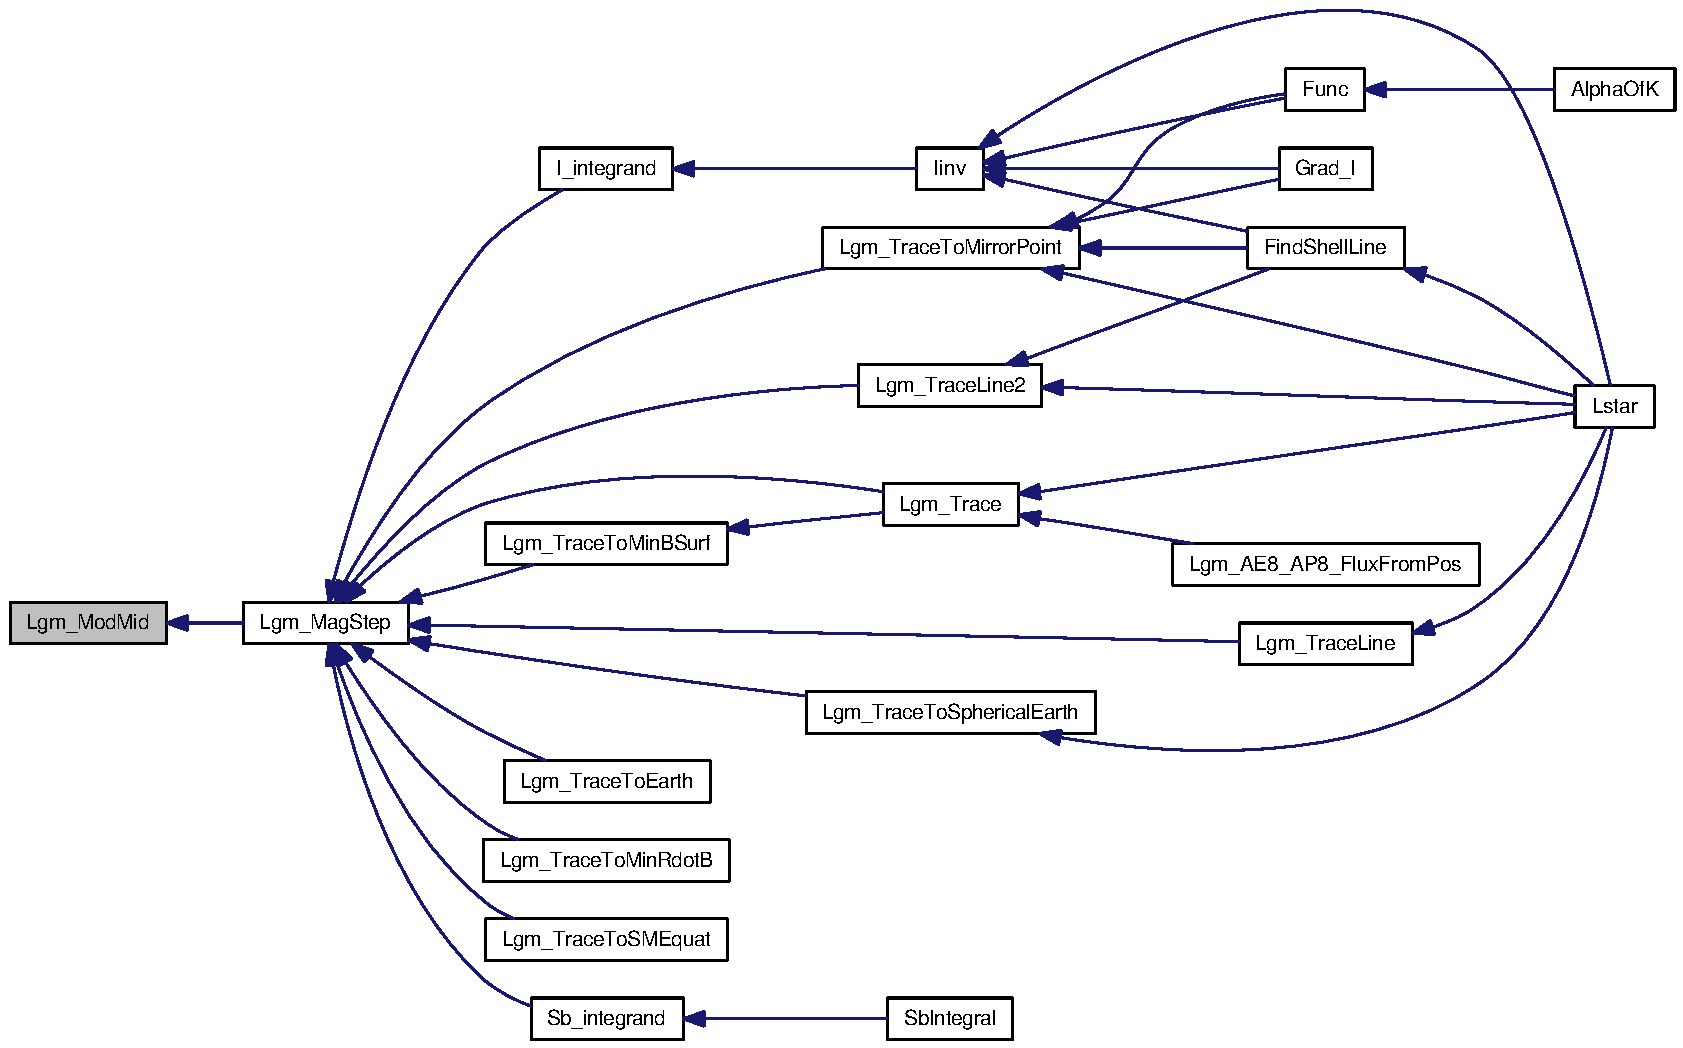
\includegraphics[width=420pt]{_mag_step_8c_25b0aafbfa7b08a20caa7103067395eb_icgraph}
\end{center}
\end{figure}
\hypertarget{_mag_step_8c_e3bb72fc4563ef180d82d4cc003bcf0e}{
\index{MagStep.c@{MagStep.c}!Lgm\_\-RatFunExt@{Lgm\_\-RatFunExt}}
\index{Lgm\_\-RatFunExt@{Lgm\_\-RatFunExt}!MagStep.c@{MagStep.c}}
\subsubsection[{Lgm\_\-RatFunExt}]{\setlength{\rightskip}{0pt plus 5cm}void Lgm\_\-RatFunExt (int {\em k}, \/  double {\em x\_\-k}, \/  {\bf Lgm\_\-Vector} $\ast$ {\em u\_\-k}, \/  {\bf Lgm\_\-Vector} $\ast$ {\em w}, \/  {\bf Lgm\_\-Vector} $\ast$ {\em dw}, \/  {\bf Lgm\_\-MagModelInfo} $\ast$ {\em Info})}}
\label{_mag_step_8c_e3bb72fc4563ef180d82d4cc003bcf0e}




Definition at line 85 of file MagStep.c.

Here is the caller graph for this function:\nopagebreak
\begin{figure}[H]
\begin{center}
\leavevmode
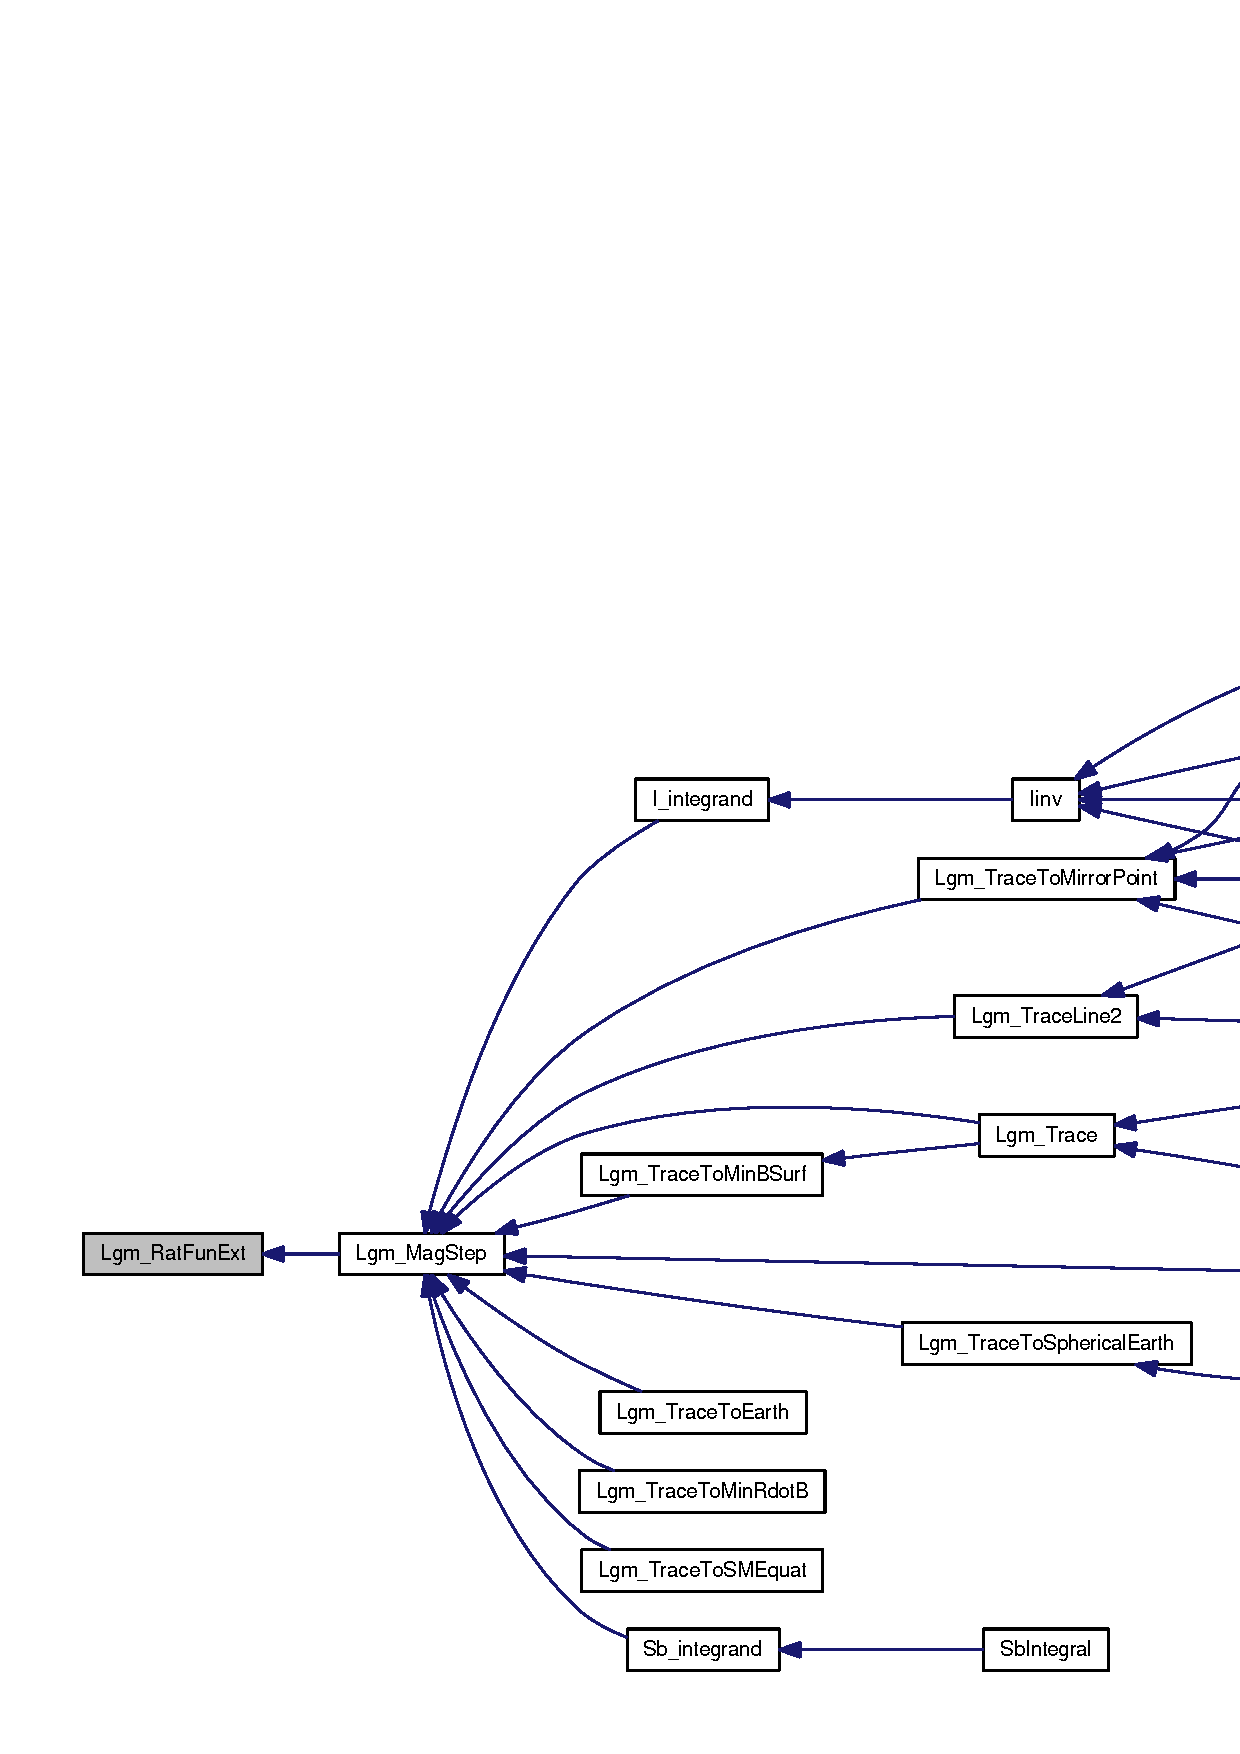
\includegraphics[width=420pt]{_mag_step_8c_e3bb72fc4563ef180d82d4cc003bcf0e_icgraph}
\end{center}
\end{figure}
\hypertarget{_mag_step_8c_3b19333caf8b3d06e1b4c54e4473096b}{
\index{MagStep.c@{MagStep.c}!Lgm\_\-MagStep@{Lgm\_\-MagStep}}
\index{Lgm\_\-MagStep@{Lgm\_\-MagStep}!MagStep.c@{MagStep.c}}
\subsubsection[{Lgm\_\-MagStep}]{\setlength{\rightskip}{0pt plus 5cm}int Lgm\_\-MagStep ({\bf Lgm\_\-Vector} $\ast$ {\em u}, \/  {\bf Lgm\_\-Vector} $\ast$ {\em u\_\-scale}, \/  double {\em Htry}, \/  double $\ast$ {\em Hdid}, \/  double $\ast$ {\em Hnext}, \/  double {\em eps}, \/  double {\em sgn}, \/  double $\ast$ {\em s}, \/  int $\ast$ {\em reset}, \/  int($\ast$)({\bf Lgm\_\-Vector} $\ast$, {\bf Lgm\_\-Vector} $\ast$, {\bf Lgm\_\-MagModelInfo} $\ast$) {\em Mag}, \/  {\bf Lgm\_\-MagModelInfo} $\ast$ {\em Info})}}
\label{_mag_step_8c_3b19333caf8b3d06e1b4c54e4473096b}




Definition at line 157 of file MagStep.c.

Here is the call graph for this function:\nopagebreak
\begin{figure}[H]
\begin{center}
\leavevmode
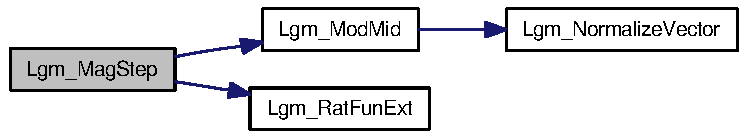
\includegraphics[width=197pt]{_mag_step_8c_3b19333caf8b3d06e1b4c54e4473096b_cgraph}
\end{center}
\end{figure}


Here is the caller graph for this function:\nopagebreak
\begin{figure}[H]
\begin{center}
\leavevmode
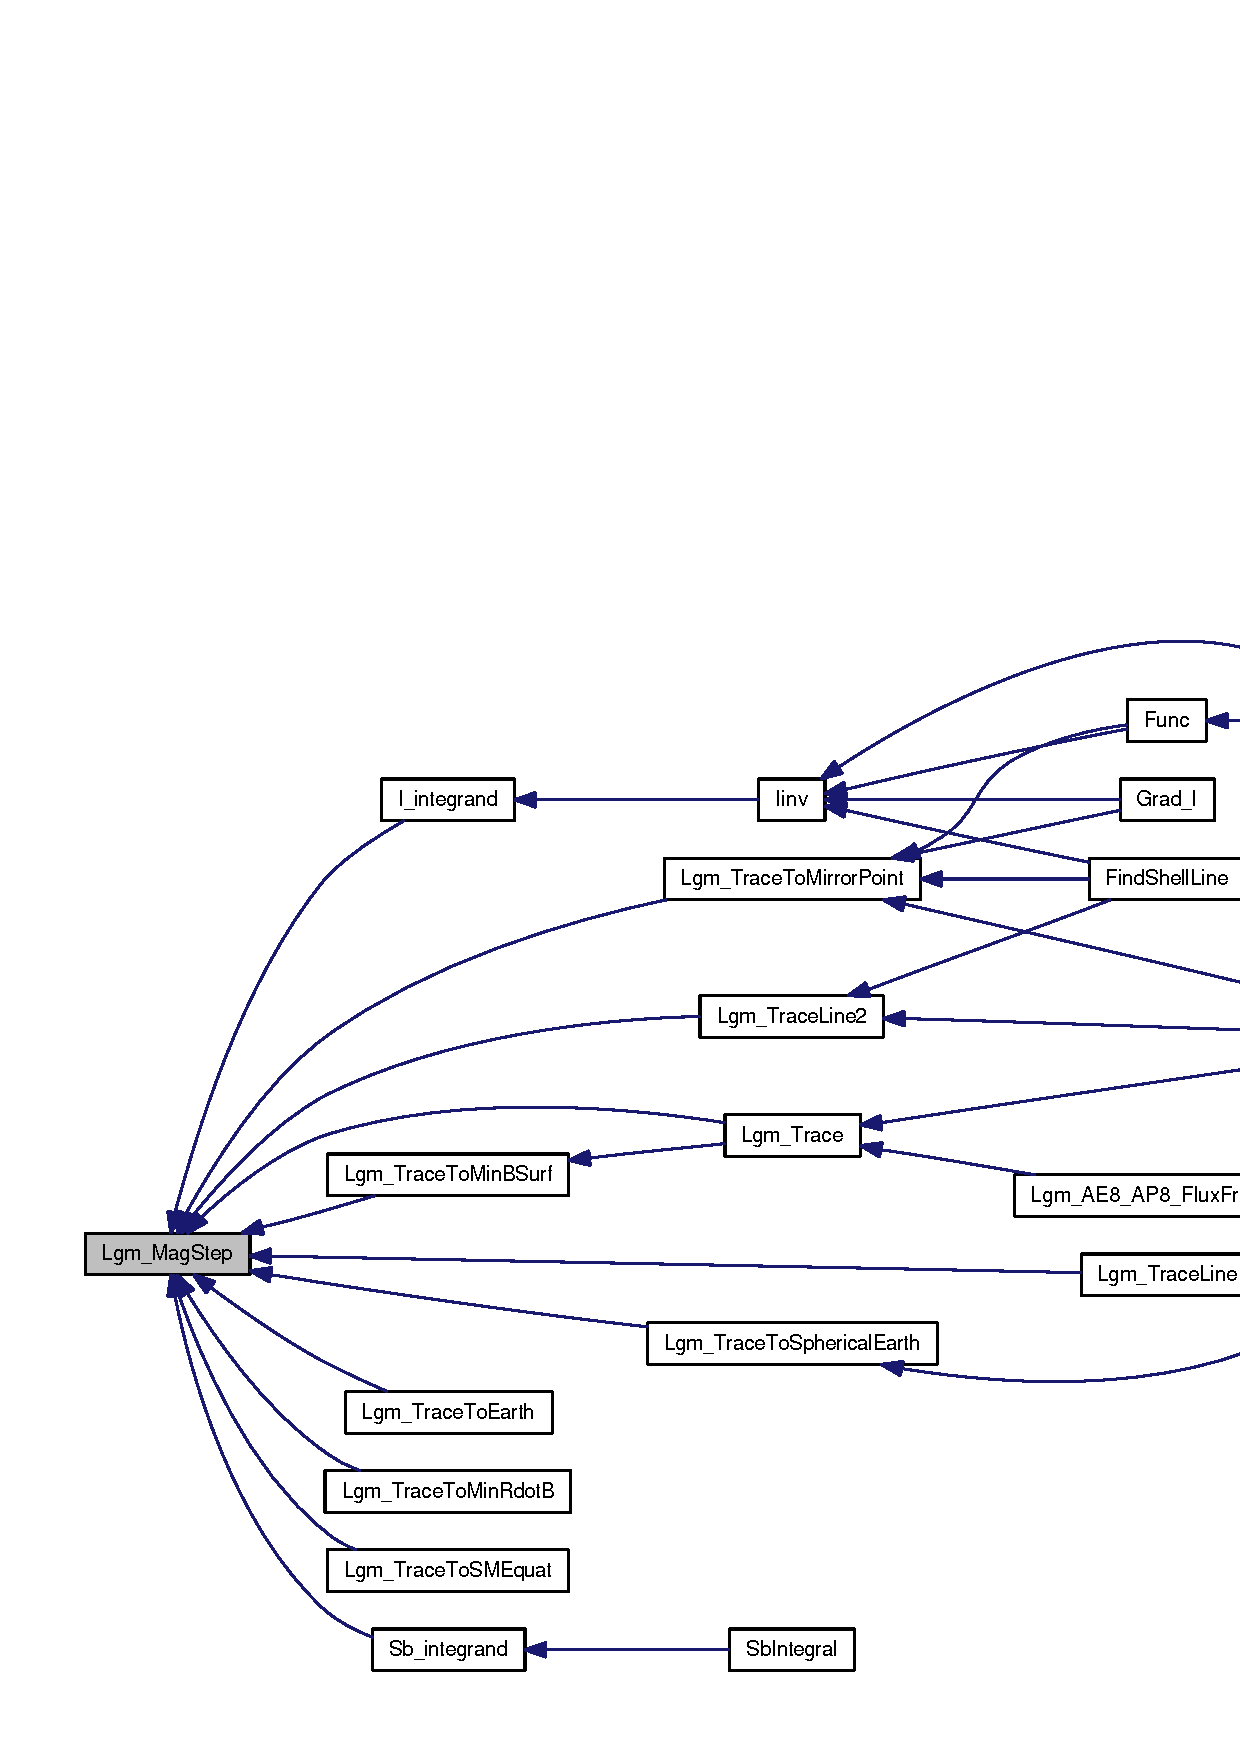
\includegraphics[width=366pt]{_mag_step_8c_3b19333caf8b3d06e1b4c54e4473096b_icgraph}
\end{center}
\end{figure}
